%%============
%%  ** Author: Shepherd Qirong
%%  ** Date: 2021-12-11 17:07:45
%%  ** Github: https://github.com/ShepherdQR
%%  ** LastEditors: Shepherd Qirong
%%  ** LastEditTime: 2021-12-11 17:23:55
%%  ** Copyright (c) 2019--20xx Shepherd Qirong. All rights reserved.
%%============



\documentclass[UTF8]{article}
\usepackage{ctex}
\usepackage{amsmath,amsthm,amsfonts,amssymb,bm,mathrsfs,upgreek} 
\usepackage{graphicx}
\usepackage[paper=a4paper,top=3.5cm,bottom=2.5cm,
left=2.7cm,right=2.7cm,
headheight=1.0cm,footskip=0.7cm]{geometry}
\usepackage{color}
\usepackage{multirow,booktabs}

\RequirePackage{setspace}%%linespace
\setstretch{1.523}


\begin{document}
\section{Introduction}
Today is 20211211, and I deciede to note down all of my knowledge about problems in this notebook. Actually we think for a while whether to seperatre the knowledge into different documents.

\section{Physics}

\subsection{Energy}

\subsubsection{T0001}
The coordinate of free fall ball ends. With energy equation, we have $GH = \mu G \xi kH$, considering of the backward length, we draw the figure and it can be transfered from the figure $y = |x|$. We have the coordinate
at $[1-\vert (\mu k)^{-1} \pmod 2 -1 \vert ]kH $.
\begin{figure*}[h]
    \centering
    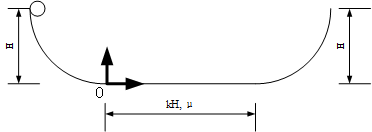
\includegraphics[width=0.5\textwidth]{../../resources/T0001.png}
    \caption{[T0001: Where the ball ends]}
    \label{fig:1}
\end{figure*}




\end{document}